
\documentclass{acm_proc_article-sp}
\makeatletter
\newif\if@restonecol
\makeatother
\let\algorithm\relax
\let\endalgorithm\relax
\usepackage{hyperref}
\usepackage[all]{hypcap}
\usepackage[usenames,dvipsnames]{xcolor}
\usepackage{listings}
\usepackage{algorithm2e}
\hypersetup{
  bookmarks=true,         % show bookmarks bar?
  unicode=false,          % non-Latin characters in Acrobat’s bookmarks
  pdftoolbar=true,        % show Acrobat’s toolbar?
  pdfmenubar=true,        % show Acrobat’s menu?
  pdffitwindow=false,     % window fit to page when opened
  pdfstartview={FitH},    % fits the width of the page to the window
  pdftitle={My title},    % title
  pdfauthor={Author},     % author
  pdfsubject={Subject},   % subject of the document
  pdfcreator={Creator},   % creator of the document
  pdfproducer={Producer}, % producer of the document
  pdfkeywords={keyword1} {key2} {key3}, % list of keywords
  pdfnewwindow=true,      % links in new window
  colorlinks=true,       % false: boxed links; true: colored links
  linkcolor=cyan,          % color of internal links (change box color with linkbordercolor)
  citecolor=green,        % color of links to bibliography
  filecolor=magenta,      % color of file links
  urlcolor=cyan           % color of external links
}




\usepackage{listings}
\usepackage{algorithm2e}
\usepackage{verbatim}
\begin{document}
\title{Analysis of Security-Cost Trade-off of Fully Homomorphic Encryption Schemes}


%
% You need the command \numberofauthors to handle the 'placement
% and alignment' of the authors beneath the title.
%
% For aesthetic reasons, we recommend 'three authors at a time'
% i.e. three 'name/affiliation blocks' be placed beneath the title.
%
% NOTE: You are NOT restricted in how many 'rows' of
% "name/affiliations" may appear. We just ask that you restrict
% the number of 'columns' to three.
% Because of the available 'opening page real-estate'
% we ask you to refrain from putting more than six authors
% (two rows with three columns) beneath the article title.
% More than six makes the first-page appear very cluttered indeed.
%
% Use the \alignauthor commands to handle the names
% and affiliations for an 'aesthetic maximum' of six authors.
% Add names, affiliations, addresses for
% the seventh etc. author(s) as the argument for the
% \additionalauthors command.
% These 'additional authors' will be output/set for you
% without further effort on your part as the last section in
% the body of your article BEFORE References or any Appendices.

\numberofauthors{2} %  in this sample file, there are a *total*
% of EIGHT authors. SIX appear on the 'first-page' (for formatting
% reasons) and the remaining two appear in the \additionalauthors section.
%
\author{
\alignauthor
Kais Chaabouni \\
       \affaddr{ENSIMAG}\\
       \affaddr{Grenoble INP}\\
       \affaddr{Grenoble, France}\\
       \email{kais.chaabouni@ensimag.imag.fr}
% 2nd. author
\alignauthor 
Amrit Kumar\\
       \affaddr{ENSIMAG-Ecole Polytechnique}\\
       \affaddr{Grenoble INP}\\
       \affaddr{Grenoble, France}\\
       \email{amrit.kumar@ensimag.imag.fr}
}

% There's nothing stopping you putting the seventh, eighth, etc.
% author on the opening page (as the 'third row') but we ask,
% for aesthetic reasons that you place these 'additional authors'
% in the \additional authors block, viz.

\date{30 July 1999}
% Just remember to make sure that the TOTAL number of authors
% is the number that will appear on the first page PLUS the
% number that will appear in the \additionalauthors section.
\maketitle
\begin{abstract}
This paper presents an analysis of security-cost trade-off for homomorphic encryption schemes. Analysis is based on the measurements taken on the evaluation of certain functions on two  variants of fully homomorphic encryption schemes. These functions either operate on bits, on integers (of bounded and unbounded size)  or involve \texttt{if-then-else} branching. 
\end{abstract}

\keywords{ Fully Homomorphic Encryption, Security, Cost.} % NOT required for Proceedings

\section{Introduction(1 page)}

The notion of \textit{fully homomorphic encryption scheme}, orginally called a \textit{privacy homomorphism} was introduced by Rivest et al. \cite{rivest78} shortly after the invention of the RSA by Rivest, Shamir and Adleman \cite{Rivest78amethod}.  Basic RSA is a multiplicative homomorphic encryption scheme -- i.e. given the public parameters $pk:=(e, N)$ and two messages $m_0, m_1$, their encryption $c_0, c_1$ verify $c_0c_1=(m_0m_1)^e \ \textrm {mod}\ N$. With a fully homomorphic encryption scheme : a scheme $\mathcal{E}$ with an efficient algorithm $Eval_\mathcal{E}$ that evaluates any circuit $C$ on any ciphertexts $c_i \leftarrow Encrypt(pk, m_i)$; one can arbitrarily compute any function on encrypted data without the decryption key. However prior to \cite{homenc}, we did not have a viable construction.

As an application, such schemes can be used to query data on a remote machine. A user prepares his encrypted data $c_0, c_1, \ldots, c_{n-1}$  and a description of the function(or a query) i.e. a circuit $C$ he wants to evaluate and sends them to the remote machine. The machine transforms the circuit into $C^{'}$ so that it can evaluate the same function but on encrypted data, performs the operation and returns the encrypted result to the user. The user eventually decrypts the result.  

The homomorphic encryption scheme proposed by Gentry \cite{homenc} is based on ideal lattices which allows operations on encrypted data
but with a high cost depending on the depth of the circuit representing the $Eval$ function. Since then, researchers have improved and proposed other schemes such as \cite{cryptoeprint:2009:571} and \cite{cryptoeprint:2011:277} which decrease the circuit complexity. In this article we expermentally evaluate implementation of these two schemes and analyze the cost-security trade-off for $Eval$ varying from \texttt{XOR} of the bits of an $n$ bit integer to sum of bounded and unbounded integers to sorting of $n$ integers. Three different sorting algorithms are tested.   

In this article we study the implementation of basic classes of operations and different aspects of 
complexity-security, and we discuss the results of experimental measures based on several parameters.\\
The Gentry FHE protocol consists on ``somewhat homomorphic'' scheme, ``squashing'' and ``bootstrapping''. (explain later). 
There are variants of FHE schemes more optimized than Gentry's scheme, so we use in the experiments some open source implementations of these schemes.
\section{Fully homomorphic scheme(1 page)}
A general structure of the scheme.
\subsection{Two Variants of Fully Homomorphic Encryption Scheme}
A brief description of the two FHE schemes with their algorithmic complexity of the different stages in the scheme. 
-> Smart Vercauteren
-> BGV
Discuss the security of these schemes.



\begin{itemize}
\item Smart-Vercauteren scheme:\\
The scheme \cite{cryptoeprint:2009:571} has 3 parameters: ($N, \nu, \mu$ ). The somewhat homomorphic scheme uses 5 algorithms: (\texttt{KeyGen}, \texttt{Encrypt}, \texttt{Decrypt}, \texttt{Add}, \texttt{Mult}).
\begin{itemize}
\item \texttt{KeyGen}:
\begin{itemize}
\item $F(x)= x^{n}+1$
\item do
\begin{itemize}
\item $S(x)=_{R}(B_{\infty , N}(\nu/2)$
\item $G(x)=1+2.S(x)$
\item $p= resultant(G(x),F(x))$
\end{itemize}
until $p$ is prime
\item $D(x)=gcd(G(x),F(x))$ over $\mathbb{F}_p[x]$
\item $\alpha$: the unique root of $D(x)$
\item apply \texttt{fmpz\_poly\_xgcd} to obtain $Z(x)$ such that $Z(x).G(x)=p$ mod $F(x)$
\item $B=z_0$ mod $2p$
\item $PK = (p, \alpha)$ and $Sk = (p , B)$
\end{itemize}
\item \texttt{Encrypt}($m \in \{0,1\} , PK$):
\begin{itemize}
\item $R(x)=_{R}(B_{\infty , N}(\mu/2)$
\item $C(x)=m+2.R(x)$
\item $c=C(\alpha) mod p$
\item return $c$
\end{itemize}
\item \texttt{Decrypt}($c, SK$):
\begin{itemize}
\item $m= (c - round(c.B/p)) mod 2$
\item return $m$
\end{itemize}
\item \texttt{Add}($c_1$, $c_2$, $PK$):
\begin{itemize}
\item $c_3=c_1+c_2 mod p$
\item return $c_3$
\end{itemize}
\item \texttt{Mult}($c_1$, $c_2$, PK):
\begin{itemize}
\item $c_3=c_1.c_2 mod p$
\item return $c_3$
\end{itemize}
\end{itemize}
\item BGV:
\end{itemize}
\subsection{Considered Implementations}

The library used, version, implementaion details, versions, references, modifications required, how-to-installl, how-to-use.Platforms accepted and other depedeices.\\
For the Smart-Vercauteren implementation we use the library libScarab v1.0.0 which requires the following libraries: GMP, FLINT, MPIR, MPFR.
\subsection{Intial set-up cost(The cost not depending on the actual program)}

Can be integrated with subsection 2.1 

\section{ Didactic example :  Min-Max (1 page)}
Min-Max of sequence of n-btis with arithmetic operations and without branching.
\subsection{Input Program for Fully Homomorphic Encryption Scheme}


\restylealgo{algoruled}

\linesnumbered

\begin{algorithm}[H]

\SetVline

 \KwData{a':=$(a_0',a_1',\ldots, a_{n-1}'$), b':=$(b_0',b_1',\ldots, b_{n-1}')$ }

 \KwResult{Return Max(a',b') and Min(a',b')}

 $aIsGreater \leftarrow 0$\;
 $bitsEqual \leftarrow 1$\;
	
 \For{$i\leftarrow n-1 $ \KwTo $0$}{
						
     $aIsGreater \leftarrow (aIsGreater +\neg(b_i')a_i')* bitEqual$ \;
     $bitEqual \leftarrow bitEqual*(a_i'b_i' + \neg(a_i)'*\neg(b_i'))$		       	
 }

\For{$i\leftarrow 0$ \KwTo $n-1$}{

     $Max_i \leftarrow aIsGreater*a_i' + \neg(aIsGreater)*b_i'$ \;

     $Min_i \leftarrow  \neg(aIsGreater)*a_i' + aIsGreater*b_i'$ \;

 }



return($Max$, $Min$)

 \caption{Min-Max on ciphertext \label{Code:algo}}


\end{algorithm}


\subsection{Theoretical Cost with the Schemes}

The cost \texttt{aIsGreater} is:\\
 $2*encrypt+n*(3*encrypt+7*add+7*mul)$ .\\
The cost of this algorithm \texttt{min\_max} is:\\
$ encrypt+aIsGreater+2*n*(encrypt+3add+3mull)$\\
Thus this algorithm has $\theta(n)$ complexity. 

\subsection{Experimental Analysis}

Measurements taken are CPU time, Wall Time, Memory Usage by varying the input size  and the algorithmic parameters. Noise reduction threshold.\\
Here we estimate the performance of this program in terms of run time for KeyGen, Encrypt, Decrypt and the Min-Max algorithm.
\begin{itemize}

\item KeyGen\\
The measured time execution for KeyGen($N, \mu$)  for fixed values of parameters: $N=8$ and $\mu = 4$ show a variation from 0.2 s to 14.41 s with big density at the interval [0.2s, 1s].\\
\begin{figure}[!h] %on ouvre l'environnement figure
\centering
\includegraphics[width=5cm]{f3.eps} 
\caption{Run time of KeyGen(ms)} 
\label{image_f2} %l'étiquette pour faire référence à cette image
\end{figure}
\item {Encryption and Decryption}\\


\item {Cost time of Min-Max program}\\
We measure the run time from $n=1$ to $32$ bits,we find a linear cost which confirms the $\theta(n)$ complexity. During these measures the result of Min-Max is correct. 
\begin{figure}[!h] %on ouvre l'environnement figure
\centering
\includegraphics[width=5cm]{f2.eps} 
\caption{Run time(ms)} 
\label{image_f2} %l'étiquette pour faire référence à cette image
\end{figure}

\item The cost of this algorithm on ciphertext is linear with bit number, like  the algorithm on plaintext, the extra cost in this case is encryption-decryption cost and especially the code generation which is very inpreductible and take often a long time in the SV-Scheme.
\end{itemize}
\section{Choice of Benchmarks}

The benchmark problems on which the implementations were evaluated are categorized into three classes : functions operating on bits, functions operating directly on integers or block of bits and functions where branching is required i.e \texttt{if-then-else} condition is evaluated. 

Functions operating on bits provide information on the tradeoff for bitwise operations, while when operating directly on integers, the tradeoff is obtained as a function of the size of integers. The first two categories of functions can be evaluated using straight-line programs. For others, evaluation of \texttt{if-then-else} condition on encrypted data is choosen.  The evaluation circuit in this case is longer than the one on non-encrypted data. Hence, this provides information on increase in size of the circuit(when passing from non-encrypted to enrypted data). The addressed problems are : 

1. \textbf{XOR of bits}\\
2. \textbf{Sum of :}  
\newline\noindent
\phantom{x}\hspace{3ex} a) bounded integers 
 b) unbounded integers\\ 
3. \textbf{Majority bit} \\
4. \textbf{Sorting : } \newline\noindent
\phantom{x}\hspace{3ex} a) Insertion sort b) Oddd-Even Merge sort \\
	\phantom{x}\hspace{3ex} 	    c) Bitonic sort 

The implementations are evaluated on different sorting algorithms to compare the changes in the evaluation circuits.

\subsection{Theoretical Size of Evaluation Circuit}
As the implementations provide addition and multiplicaion of ciphertexts,  size in terms of \texttt{XOR} and \texttt{AND} gates are provided for each problem. 

\textbf{XOR of $n$-bits :} \texttt{XOR} of $n$-bits requires $n-1$ \texttt{XOR} gates. 

\textbf{Sum of integers of $n$-bits :} Sum of two integers is performed using an $n$ \texttt{full-adder} circuits. The cost of a full adder circuit is $2$ \texttt{XOR} to calculate the sum and $2$ \texttt{AND}, $1$ \texttt{XOR} and $1$ \texttt{OR} for the carry. Hence the total complexity is $3n$ \texttt{AND}, $5n$ \texttt{XOR}. 

\textbf{Sum of arbitrary integers}

\textbf{Majority of $n$-bits :} Majority bit is evaluated by obtaining the sum of the bits.

\textbf{Sorting :}
Sorting is tested on a sorting network where comparator gates are used. Each comparator is designed using the following algorithm. 

\restylealgo{algoruled}

\linesnumbered

\begin{algorithm}[H]

 \SetVline

 \KwData{a:=$(a_0,a_1,\ldots, a_{n-1}$), b:=$(b_0,b_1,\ldots, b_{n-1})$ }

 \KwResult{Return Max(a,b) and Min(a,b)}

 $aIsGreater \leftarrow 0$\;
 $bitsEqual \leftarrow 1$\;

	
 \For{$i\leftarrow n-1 $ \KwTo $0$}{
						
     $aIsGreater \leftarrow (aIsGreater +\neg(b_i)a_i)* bitEqual$ \;
     $bitEqual \leftarrow bitEqual*(a_ib_i + \neg(a_i)*\neg(b_i))$		       	
 }

\For{$i\leftarrow 0$ \KwTo $n-1$}{

     $Max_i \leftarrow aIsGreater*a_i + \neg(aIsGreater)*b_i$ \;

     $Min_i \leftarrow a \neg(aIsGreater)*a_i + aIsGreater*b_i$ \;

 }



return($Max$, $Min$)

 \caption{Comparator\label{Code:algo}}

\end{algorithm}



A comparator gate uses $n$ \texttt{AND} gates, $n$ \texttt{OR} gates and $n$ \texttt{NOT} gates to find the larger of the two bit sequences and then to regenerate the maximum and the minuimum $4n$ \texttt{AND} gates and $2n$ \texttt{NOT} and \texttt{OR} gates i.e. $6n$ \texttt{AND} and \texttt{XOR} gates are required. We note that reconstruction of Max and  Min is not required when working on non-encrypted data. Hence, this increases the size of the transformed program operating on encrypted data.

\textbf{Insertion sort :} When allowing for parallel comparators, bubble sort and insertion sort are identical. Hence $n(n-1)/2$ comparator gates are used for insertion sort.

\textbf{Odd-Even Merge sort :} \autoref{oesort} and \autoref{oemerge} are used to perform Odd-Even merge sort and hence  $n/2(log(n)-1) + 1 $ comparator gates are required. 


\textbf{Bitonic Sort :} \autoref{bitsort} and \autoref{bitmerge} are used to perform Bitonic Sort and hence $log(n) · (log(n)+1) / 2 $ gates are required.


\lstset{                                    % line wrapping on
  language=C,
  frame=lines,
  captionpos=b
 }


\renewcommand{\lstlistingname}{Code}

\section{Evaluation on the benchmarks}
Measurements by varying the parameters or the plaintext size.
\section{Analysis of the results}

Anlayze the results previously obtained and its impact on security and complexity. Comparisions of security-cost tradeoff with other schemes like RSA.
\section{Conclusion}



\bibliographystyle{alpha}
\bibliography{article}  

%\begin{comment}
\section{Appendix}

 The programs used for Odd-Even Merge sort and Bitonic sort are provided below : 


\begin{figure}[h]
\begin{lstlisting}[label = oesort ]

 OddEvenMergeSort(int lo, int n)
if (n > 1)
        {
            int m = n/2;
            oddEvenMergeSort(lo, m);
            oddEvenMergeSort(lo + m, m);
            oddEvenMerge(lo, n, 1);
        }

\end{lstlisting}
\caption{Odd-Even Merge Sort : sort from index lo to n }
\end{figure}


\begin{figure}
\begin{lstlisting}[label = oemerge ]

oddEvenMerge(int lo, int n, int r)
    {
        int m = r*2;
        if (m < n)
        {
	    //even subsequence ;		
            oddEvenMerge(lo, n, m); 
            //odd subsequence ;
	    oddEvenMerge(lo+r, n, m); 
	    int i = lo+r;   
            for (;i + r < lo + n;){
		compare(i, i + r);
		i += m;
	    }
        }
        else
            compare(lo, lo + r);
    }


\end{lstlisting} 
\caption{Odd-Even Merge Sort : merging function}
\end{figure}

\begin{figure}
\begin{lstlisting}[label=bitsort]

sortup( int m, int n) {//from m to m+n
    if (n == 1) return;
    sortup(m, n/2);
    sortdown(m + n/2, n/2);
    mergeup(m, n/2);
}
 sortdown(int m, int n) {//from m to m+n
    if (n == 1) return;
    sortup(m, n/2);
    sortdown(m + n/2, n/2);
    mergedown(m, n/2);
}
\end{lstlisting}
\caption{Bitonic Sort : sort form m to n}
\end{figure}

\begin{figure}[t]
\begin{lstlisting}[label=bitmerge]
mergeup(int m, int n) {  
    if (n == 0) return;
    
    for (i = 0 : n)
        // Increasing Comparator
	 compare(m + i,m + i + n);
    mergeup(m, n/2);
    mergeup(m + n,n/2);
}

mergedown( int m,  int n) { 
    if (n == 0) return;
    for (i = 0 : n) 
        // Decreasing Comparator
	compare(m + i, m + i + n); 
    mergedown(m, n/2);
    mergedown(m + n, n/2);
}
\end{lstlisting}
\caption{Bitonic Merge} 
\end{figure} 
%\begin{comment}


% sigproc.bib is the name of the Bibliography in this case
% You must have a proper ".bib" file
%  and remember to run:
% latex bibtex latex latex
% to resolve all references
%
% ACM needs 'a single self-contained file'!
%
%APPENDICES are optional
%\balancecolumns
\balancecolumns
% That's all folks!
\end{document}
